\newpage
\section{Animations}
Two important concepts in animations are \textbf{Quaternions} and \textbf{Bezier Curves}

\subsection{Quaternions}
When dealing with movements considering Euler angle rotations the \textbf{gimbal lock} represented an important problem : it causes to loose one degree of freedom due to the alignment of two rotating axis in the same direction. This phenomenon causes \textbf{unrealistic movements}. \textbf{Quaternions} are a solution to this problem : it encodes a rotation in space with \textbf{4 numbers} linearly dependent ( instead of 3).\\
Quaternions are \textbf{extensions} of complex numbers that have \textbf{three imaginary components}:
\begin{itemize}
\item Complex number $\rightarrow$ $a+ib$
\item Quaternions $\rightarrow$ $a+ib+jc+kd$ where the three imaginary components are called \textbf{vector part} subject to the following relation $$ i^2 + j^2 + k^2 = ijk = -1$$ $$ i \cdot j = k  $$ $$... $$
\end{itemize}
A complete algebra can be defined with Quaternions : 
\begin{itemize}
\item Sum of two quaternions $$ (a_1+ib_1+jc_1+kd_1)+(a_2+ib_2+jc_2+kd_2) = (a_1+a_2)+i(b_1+b_2)+j(c_1+c_2)+k(d_1+d_2)$$
\item Product with scalar $$ \alpha(a+ib+jc+kd)= \alpha a+i\cdot \alpha
 b + j\cdot \alpha c + k\cdot \alpha d$$
\item Product of two quaternions
 \begin{align*}
(a_1+ib_1+jc_1+kd_1)(a_2+ib_2+jc_2+kd_2) = (a_1a_2-b_1b_2-c_1c_2-d_1d_2)\\+i(a_1b_2+b_1a_2+c_1d_2-d_1c_2)\\+j(a_1c_2+c_1a_2+d_1b_2-b_1d_2)\\+k(a_1d_2+d_1a_2+b_1c_2-c_1b_2)
\end{align*}
\item Norm $$ ||a+ib+jc+kd||= \sqrt{a^2+b^2+c^2+d^2}$$
\item Angle $$ \theta = arcos\frac{a}{\sqrt{a^2+b^2+c^2+d^2}} $$
\item Rising to power $\alpha$ $$ (a+ib+jc+kd)^{\alpha}= ||a+ib+jc+kd||^{\alpha}\left( cos(\alpha \theta)+ \frac{ib+jc+kd}{\sqrt{b^2+c^2+d^2}}sin(\alpha \theta)\right)$$
\item Unitary quaternions $$ ||a+ib+jc+kd||= \sqrt{a^2+b^2+c^2+d^2} = 1$$
\end{itemize}
Quaternions can encode rotations in 3D of an angle $\theta$ along an axis oriented along a \textbf{unitary} vector $v=(x,y,z)$ : 
\[
\boxed{q= cos \frac{\theta}{2} + sin \frac{\theta}{2} (ix+jy+kz)}
\]
Since v is unitary also \textbf{q is unitary}.
For example a rotation along the x-axis only ( v= (1,0,0)):
$$ q= cos \frac{\theta}{2} + isin \frac{\theta}{2} $$
If two unitary quaternions $q_1 q_2$ encode two different rotations  then their product encodes the composed form : $$ M_1 \Leftrightarrow q_1 \quad M_2 \Leftrightarrow q_2 \to M_1 \cdot M_2 \Leftrightarrow q_1 \cdot q_2$$
This way Euler angles can be transformed into a quaternion:
$$ R = R_y(\Phi) \cdot R_x(\theta) \cdot R_z(\phi)$$
\[
\boxed{q=\left( cos \frac{\psi}{2}+jsin \frac{\phi}{2}\right) \left( cos \frac{\theta}{2}+isin \frac{\theta}{2}\right)\left( cos \frac{\phi}{2}+ksin \frac{\phi}{2}\right)}
\]
where
\begin{align*}
q= \left( cos \frac{\psi}{2} cos \frac{\theta}{2} cos \frac{\phi}{2}- sin \frac{\psi}{2}sin \frac{\theta}{2} sin \frac{\phi}{2} \right) \\
+i\left( cos \frac{\psi}{2} sin \frac{\theta}{2} cos \frac{\phi}{2}- sin \frac{\psi}{2}cos \frac{\theta}{2}sin\frac{\phi}{2}\right) \\
+j \left( sin \frac{\psi}{2} cos \frac{\theta}{2} cos \frac{\phi}{2}- cos \frac{\psi}{2}sin \frac{\theta}{2}sin\frac{\phi}{2}\right)\\
+k \left( cos \frac{\psi}{2} sin \frac{\theta}{2} cos \frac{\phi}{2}- sin \frac{\psi}{2}sin \frac{\theta}{2}cos\frac{\phi}{2}\right)
\end{align*}
The opposite operation where $q=a+ib+jc+kd$ can be easily converted into a \textbf{rotation matrix} :

$$ R= \begin{bmatrix}
    1-2c^2-2d^2       & 2bc+2ad & 2bd-2ac  & 0 \\
    2bc-2ad      & 1-2b^2-2d^2 & 2cd+ 2ab & 0 \\
    2bd+2ac       & 2cd-2ab & 1-2b^2-2c^2 & 0 \\
    0 & 0 & 0 & 1 
\end{bmatrix}$$

\subsection{Bezier Curves}
Bezier curves are \textbf{non-linear interpolation technique} that uses several intermediate points to control the shape of the curve.Their are characterized by their degree : \textbf{linear} ,\textbf{quadratic} , \textbf{cubic}...\\
Bezier curves of degree N are defined by \textbf{N+1 values} and are computed in a \textbf{recursive} way. Consider a  linear interpolation ( function similar to the one see in the first chapters ) between two values a and b at intermediate point $\alpha \in [0,1]$ $$ lerp(a,b,\alpha )=  (1-\alpha)a+\alpha b = I(0,\alpha,1,a,b )$$
A Bezier curved of degree N defined by points $x_0,...,x_N$ passes in $x_0 \text{ at } \alpha =0 $ and in $x_N \text{ at } \alpha =1$ . The function $Bezier_n(x_0,...,x_N,\alpha)$ returns the value of the Bezier curve of degree n at intermediate point $\alpha$ :
\[
\boxed{Bezier_1(x_0,x_1,\alpha)=lerp(x_0,x_1,\alpha)}
\]
\[
\boxed{Bezier_N(x_0,...,x_N,\alpha)= lerp(Bezier_{N-1}(x_0,...,x_{N-1},\alpha),Bezier_{N-1}(x_1,...,x_{N},\alpha),\alpha) }
\]
So for N points the Bezier functions split the set in two :
\begin{itemize}
\item from $x_0 \to x_{N-1}$
\item from $x_1 \to x_{N}$ 
\end{itemize}
Then the \texttt{lerp} function with those two as first two arguments is applied.
For example in a cubic curve : 
$$ Q_0=x_{01} = lerp(x_0,x_1,\alpha)$$
$$ Q_1=x_{12} = lerp(x_1,x_2,\alpha)$$
$$ Q_3=x_{23} = lerp(x_2,x_3,\alpha)$$
$$ R_0=x_{012} = lerp(x_{01},x_{12},\alpha)$$
$$ R_1=x_{123} = lerp(x_{12},x_{23},\alpha)$$
$$ B=Bezier(x_0,x_1,x_2,x_3,\alpha) = lerp(x_{012},x_{123},\alpha)$$
 \begin{figure}[H]
 \centering
 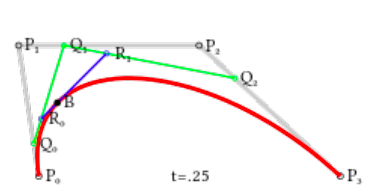
\includegraphics[width=.5\linewidth]{bezier} 
 \end{figure}
The procedure is done with a constant interpolating value $\alpha$ repeated several times.
The control points can be factorized in polynomial form :
$$ Bezier_n(x_0,...,x_N, \alpha) = \sum\limits_{i=0}^{n} \binom{n}{i}(1-\alpha)^{n-1}\alpha^ix_i $$
\[
\boxed{Bezier_2(x_0,x_1,x_2,\alpha) = (1-\alpha)^2x_0+2(1-\alpha)\alpha x_1+\alpha^2 x_2} 
\]
\[
\boxed{Bezier_2(x_0,x_1,x_2,x_3,\alpha) = (1-\alpha)^3x_0+3(1-\alpha)^2 \alpha x_1+3(1-\alpha)^2 \alpha x_2+\alpha^3 x_3} 
\]

\subsection{3D Animation}
The aim of 3D animation is to reproduce the motion of objects. The scene is divided into a set of images (\textbf{frames}) recorded at a given speed (\textbf{frames per second}). To guarantee \textbf{persistence of vision} FPS are at least \textbf{24} so that the user perceives the animation as a continuous flow. While the synchronization between recorded images and the reproduction is \textbf{natural in movies} ,it is \textbf{not} in computer graphics : this is because the speed at which the display shows the images is usually faster than the one at which the animation is created. To overcome this issue all frames are \textbf{interpolated} to create a continuous evolution of the objects of the scene. \\ 3D animation uses the \textbf{key-frame technique}:
\begin{enumerate}

\item First the important scenes are drawn 
 \begin{figure}[H]
 \centering
 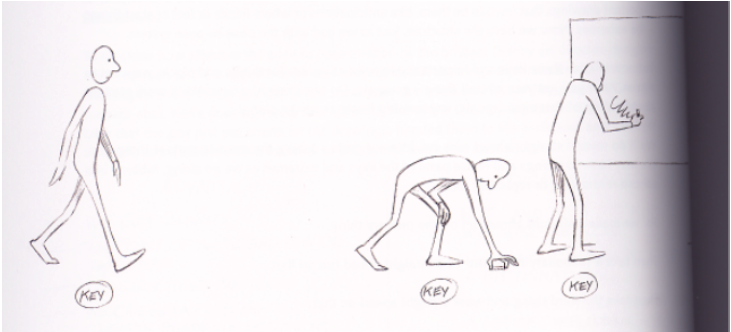
\includegraphics[width=.5\linewidth]{animation1} 
 \end{figure}
\item Then the \textbf{extreme points} are drawn  (where short-time equilibrium are reached)
 \begin{figure}[H]
 \centering
 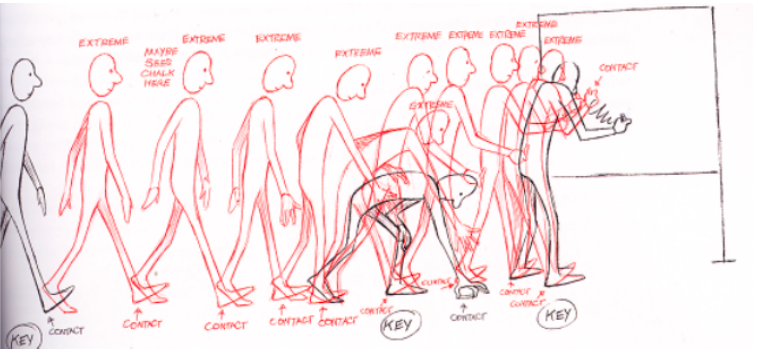
\includegraphics[width=.5\linewidth]{animation2} 
 \end{figure}
\item \textbf{Breakdown} poses that defined speed and acceleration
 \begin{figure}[H]
 \centering
 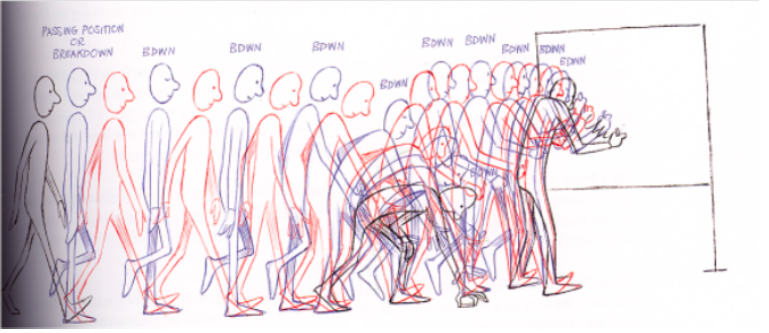
\includegraphics[width=.5\linewidth]{animation3} 
 \end{figure}
\item Finally the frames between the breakdown poses (\textbf{in-between poses}) are drawn
 \begin{figure}[H]
 \centering
 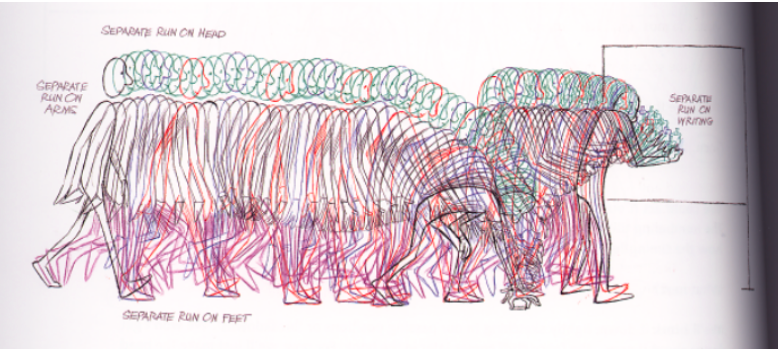
\includegraphics[width=.5\linewidth]{animation4} 
 \end{figure}
\end{enumerate} 
In computer animation the \textbf{animator} takes care of \textbf{steps 1 - 3} while the last step 4 (in-between poses) are generated through \textbf{interpolation}. This allows to: 
\begin{itemize}
\item Use \textbf{less memory }as the poses are stored only every few frames
\item Be \textbf{speed independent} as interpolating creates a continuous flow which can be sampled at un-even intervals according to the playback speed and regardless of the frame rate at which the animation was defined.
\item  \textbf{reduce animation authoring time} as artists do not have to manually create all frames.
\end{itemize}
Storing all the \textbf{parameters} for animation requires a lot of memory space , which often cannot be afforded. Moreover many parameters \textbf{don't change} during the animation (like time scaling or colors which remain constant). Only the values that change over time are stored : these parameters are called \textbf{animation channels} (for example the x position of a car is an animation channel). Frame in which such parameters are defined are called \textbf{key-frames}. Values of parameters in the key-frames \textbf{cannot be interpolated linearly} : the human eye is too \textbf{sensitive} to speed changes and linear interpolation would create such\textbf{ speed discontinuities } which would make the animation appear blocky. This is why 3D animation uses \textbf{Bezier curves of third degree} : this allows to define for each key frame the \textbf{value of the parameters} and its \textbf{first derivative} ( allows to have continuity in \textbf{position} and \textbf{velocity}!). The role of the animator is to work on the intermediate points.\\ Rotations in animations are done using \textbf{quaternions} which are not subject gimbal lock and thus allow smooth movements. Usually the following steps are adopted in computer graphics : 
\begin{enumerate}
\item Initial rotation of the object (key-frames or application generated data), are encoded using \textbf{Euler angles}.
\item Whenever they have to be \textbf{animated} Euler angles are transformed into \textbf{quaternions}
\item \textbf{Interpolation} or updates to the angles are performed on the angles
\item \textbf{Rotation matrices} are computed from the quaternion ,encoding the final orientations of the objects
\item If Euler angles need to be computed from intermediate frames they are extracted from the quaternions
\end{enumerate}
\textbf{Quaternion interpolation} has better results than \textbf{Euler interpolation} but requires some special kinds of interpolation:
\begin{itemize}
\item \texttt{nLerp} \textbf{Normalized Linear Interpolation}
\item \texttt{sLerp} \textbf{Spherical Linear Interpolation}
\end{itemize}
To obtain optimal results these techniques are combined with \textbf{Bezier curves}.